%%%%%%%%%%%%%%%%%%%%%%%%%%%%%%%%%%%%%%%%%
% Beamer Presentation
% LaTeX Template
% Version 1.0 (10/11/12)
%
% This template has been downloaded from:
% http://www.LaTeXTemplates.com
%
% License:
% CC BY-NC-SA 3.0 (http://creativecommons.org/licenses/by-nc-sa/3.0/)
%
%%%%%%%%%%%%%%%%%%%%%%%%%%%%%%%%%%%%%%%%%

%----------------------------------------------------------------------------------------
%	PACKAGES AND THEMES
%----------------------------------------------------------------------------------------

\documentclass{beamer}

\mode<presentation> {

% The Beamer class comes with a number of default slide themes
% which change the colors and layouts of slides. Below this is a list
% of all the themes, uncomment each in turn to see what they look like.

%\usetheme{default}
%\usetheme{AnnArbor}
%\usetheme{Antibes}
%\usetheme{Bergen}
%\usetheme{Berkeley}
%\usetheme{Berlin}
%\usetheme{Boadilla}
%\usetheme{CambridgeUS}
%\usetheme{Copenhagen}
%\usetheme{Darmstadt}
%\usetheme{Dresden}
%\usetheme{Frankfurt}
%\usetheme{Goettingen}
%\usetheme{Hannover}
%\usetheme{Ilmenau}
%\usetheme{JuanLesPins}
%\usetheme{Luebeck}
\usetheme{Madrid}
%\usetheme{Malmoe}
%\usetheme{Marburg}
%\usetheme{Montpellier}
%\usetheme{PaloAlto}
%\usetheme{Pittsburgh}
%\usetheme{Rochester}
%\usetheme{Singapore}
%\usetheme{Szeged}
%\usetheme{Warsaw}

% As well as themes, the Beamer class has a number of color themes
% for any slide theme. Uncomment each of these in turn to see how it
% changes the colors of your current slide theme.

%\usecolortheme{albatross}
%\usecolortheme{beaver}
%\usecolortheme{beetle}
\usecolortheme{crane}
%\usecolortheme{dolphin}
%\usecolortheme{dove}
%\usecolortheme{fly}
%\usecolortheme{lily}
%\usecolortheme{orchid}
%\usecolortheme{rose}
%\usecolortheme{seagull}
%\usecolortheme{seahorse}
%\usecolortheme{whale}
%\usecolortheme{wolverine}

%\setbeamertemplate{footline} % To remove the footer line in all slides uncomment this line
%\setbeamertemplate{footline}[page number] % To replace the footer line in all slides with a simple slide count uncomment this line

%\setbeamertemplate{navigation symbols}{} % To remove the navigation symbols from the bottom of all slides uncomment this line
}

\usepackage{graphicx} % Allows including images
\usepackage{booktabs} % Allows the use of \toprule, \midrule and \bottomrule in tables
\usepackage{tikz}
\usepackage{tkz-graph}
\usepackage{amsmath}

\usetikzlibrary{arrows.meta, positioning, quotes, shapes, fit}


\newcommand{\norm}[1]{\left\lVert#1\right\rVert}

%----------------------------------------------------------------------------------------
%	TITLE PAGE
%----------------------------------------------------------------------------------------

\title[TransE]{Translational Embeddings} % The short title appears at the bottom of every slide, the full title is only on the title page

% \author{F. Zhapa} % Your name
% \institute[KAUST] % Your institution as it will appear on the bottom of every slide, may be shorthand to save space
% {
% KAUST \\ % Your institution for the title page
% \medskip
% \textit{fernando.zhapacamacho@kaust.edu.sa} % Your email address
% }
% \date{\today} % Date, can be changed to a custom date

\begin{document}

\begin{frame}
\titlepage % Print the title page as the first slide
\end{frame}

% \begin{frame}
% \frametitle{Overview} % Table of contents slide, comment this block out to remove it
% \tableofcontents % Throughout your presentation, if you choose to use \section{} and \subsection{} commands, these will automatically be printed on this slide as an overview of your presentation
% \end{frame}

%----------------------------------------------------------------------------------------
%	PRESENTATION SLIDES
%----------------------------------------------------------------------------------------

%------------------------------------------------

\subsection{Translating embeddings}
\begin{frame}
  \frametitle{Translating embeddings}
  \begin{definition}
    Let $KG = (V, E, L; \vdash)$ be a \textbf{knowledge graph} with a set of
    vertices $V$, a set of edges $E \subseteq V \times V$, a label
    function $L: V \cup E \mapsto Lab$ that assigns labels from a set
    of labels $Lab$ to vertices and edges, and an inference relation
    $\vdash$. \textbf{A knowledge graph embedding is a function}
    $f_\eta : L(V) \cup L(E) \mapsto \mathbf{R}^n$.
  \end{definition}


  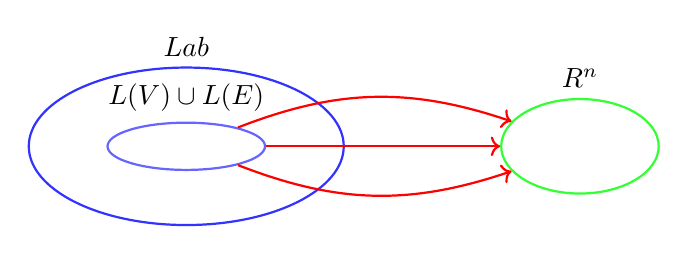
\begin{tikzpicture}[node distance=5cm, auto, thick, scale = 0.9]
    
    \node[
    ellipse,
    label = $L(V) \cup L(E)$,
    draw=blue!60,
    minimum width = 2cm, 
    minimum height = 0.6cm] (nA) {};
    
    \node[
    ellipse,
    label = $Lab$,
    draw=blue!80,
    fit=(nA),
    inner sep=1mm,
    minimum width = 4cm, 
    minimum height = 2cm] (Fit1) {};

    \pause
    \node[
    label = $\mathbb{R}^n$,
    ellipse,
    draw=green!80,
    inner sep=1mm,
    right of = Fit1,
    minimum width = 2cm, 
    minimum height = 1.2cm](real) {};

    \pause
    \draw[red, ->, bend left =20] 
        (nA) to (real);
    \draw[red, ->, bend right =20] 
        (nA) to (real);

    \draw[red, ->] 
        (nA) to (real);       

\end{tikzpicture}

\end{frame}

\begin{frame}
  \frametitle{TransE idea}

  \pause
  Graph as edgelist: set of $(h,\ell,t)$ statements\\
  \pause
  Idea: $\boldsymbol{h} + \boldsymbol{\ell} \approx \boldsymbol{t}$ (bold symbols represent embeddings)\\
  \pause
  Compute \textit{dissimilarity}: $d(\boldsymbol{h}+\boldsymbol{\ell}, \boldsymbol{t}) = \norm{\boldsymbol{h} + \boldsymbol{\ell} - \boldsymbol{t} }$ (chose your norm, usually L2)
  \pause
  
  Minimize: $$\mathcal{L}=\sum_{(h, \ell, t) \in S} \sum_{\left(h^{\prime}, \ell, t^{\prime}\right) \in S_{(h, \ell, t)}^{\prime}}\left[\gamma+d(\boldsymbol{h}+\boldsymbol{\ell}, \boldsymbol{t})-d\left(\boldsymbol{h}^{\prime}+\boldsymbol{\ell}, \boldsymbol{t}^{\prime}\right)\right]_{+}$$

\end{frame}

\begin{frame}
  \frametitle{Objective function}

  $$\mathcal{L}=\sum_{(h, \ell, t) \in S} \sum_{\left(h^{\prime}, \ell, t^{\prime}\right) \in S_{(h, \ell, t)}^{\prime}}\left[\gamma+d(\boldsymbol{h}+\boldsymbol{\ell}, \boldsymbol{t})-d\left(\boldsymbol{h}^{\prime}+\boldsymbol{\ell}, \boldsymbol{t}^{\prime}\right)\right]_{+}$$

  \begin{itemize}
    \pause
  \item $d(\boldsymbol{h}+\boldsymbol{\ell}, \boldsymbol{t})$ is score for positive edges (or triples)
    \pause
  \item $d\left(\boldsymbol{h}^{\prime}+\boldsymbol{\ell}, \boldsymbol{t}^{\prime}\right)$ is score for negative edges (or triples)
    \pause
  \item $\gamma$ is a margin parameter
    \pause
  \item $\left[ x \right]_+ = \max(0, x)$  
  \end{itemize}
  
\end{frame}

\begin{frame}
  \frametitle{Translating embeddings}
  \centerline{\includegraphics[width=.7\textwidth]{transe-figure.png}}
\end{frame}

\begin{frame}
  \frametitle{Translating embeddings}
  \begin{columns}
    \begin{column}{.6\textwidth}
      \resizebox{1\textwidth}{!}{%
        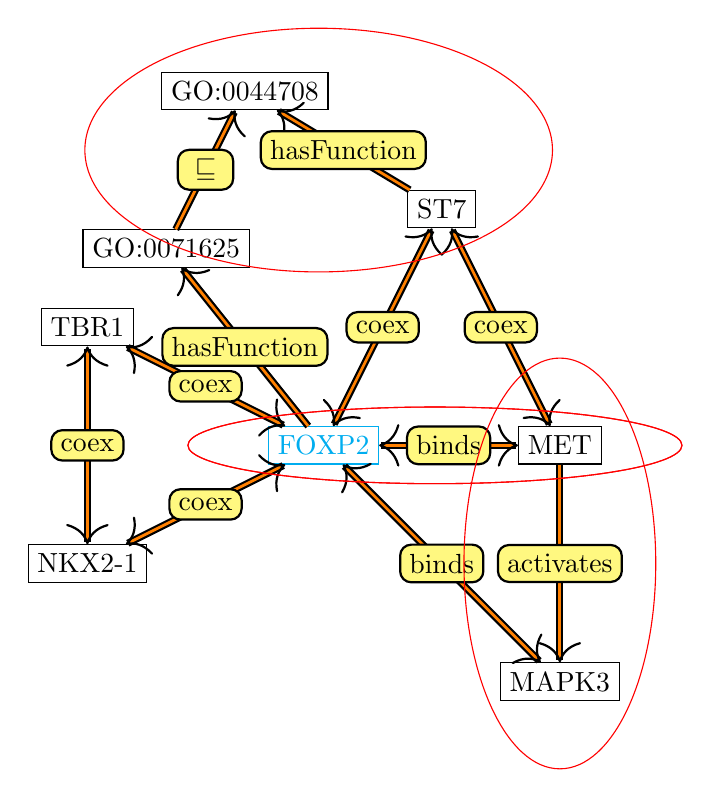
\begin{tikzpicture}
%          \SetUpEdge[lw = 1pt, color = black]
          \GraphInit[vstyle=Shade]
          \tikzset{
            LabelStyle/.style = { rectangle, rounded corners, draw,
              minimum width = 2em, fill = yellow!50,
              text = black },
            VertexStyle/.append style = { inner sep=5pt,
              font = \Large\bfseries},
            EdgeStyle/.append style = {->} }
          
          \SetGraphUnit{5}
          % \tikzset{VertexStyle/.append style={fill}}
          % \tikzset{EdgeStyle/.style={->}}
          \onslide<1->{
            \node[draw, color=cyan] (FOXP2) at (0,0) {FOXP2};
            \node[draw] (MET) at (3,0) {MET};
            \node[draw] (ST7) at (1.5,3) {ST7};
            \node[draw] (MAPK3) at (3,-3) {MAPK3};
            \node[draw] (GO0071625) at (-2,2.5) {GO:0071625};
            \node[draw] (GO0044708) at (-1,4.5) {GO:0044708};
            \node[draw] (TBR1) at (-3,1.5) {TBR1};
            \node[draw] (NKX2-1) at (-3,-1.5) {NKX2-1};
            \begin{scope}[/tikz/handle active characters in nodes=false]
              \Edge[label=activates](MET)(MAPK3)
              \Edge[label=hasFunction](FOXP2)(GO0071625)
              \Edge[label=hasFunction](ST7)(GO0044708)
              \Edge[label=$\sqsubseteq$](GO0071625)(GO0044708)
              
              \tikzset{EdgeStyle/.append style={<->}}
              \Edge[label=binds](FOXP2)(MET)
              \Edge[label=binds](FOXP2)(MAPK3)
              \Edge[label=coex](FOXP2)(TBR1)
              \Edge[label=coex](FOXP2)(NKX2-1)
              \Edge[label=coex](FOXP2)(ST7)
              \Edge[label=coex](MET)(ST7)
              \Edge[label=coex](NKX2-1)(TBR1)
            \end{scope}
          }
          % \tikzset{EdgeStyle/.style={->}}
          % \Edge[label=hf](FOXP2)(GO0044708)
          % \draw[label=binds] (FOXP2) to (MET);
          % \Edge[label=binds](FOXP2)(MET)
          % \Edge[label=activates](MET)(MAPK3)
          % \Edge[label=coexpressed-with](FOXP2)(FOXP4)
          
          \onslide<2>{
            \node[ellipse,draw=red, fit=(FOXP2) (MET),inner sep=1mm](Fit1) {};
          }

          \onslide<3>{
            \node[ellipse,draw=red, fit=(MAPK3) (MET),inner sep=1mm](Fit1) {};          
          }

          
          \onslide<4> {
            \node[ellipse,draw=red, fit=(FOXP2) (MET),inner sep=1mm](Fit1) {};
          }

          \onslide<5> {
            \node[ellipse,draw=red, fit=(ST7) (GO0044708),inner sep=1mm]() {};
          }
          

          
        \end{tikzpicture}
      }
    \end{column}
    \begin{column}{.4\textwidth}
      \begin{itemize}
      \item <2-> FOXP2 + binds = MET
        
      \item <3-> MET + activates = MAPK3
        
      \item <4-> MET + binds = FOXP2
        
      \item <5-> ST7 + hasFunction = {\tt GO:0044708}
        
      \item <6-> ...
      \end{itemize}
    \end{column}
  \end{columns}
\end{frame}

\begin{frame}
  \frametitle{Translating embeddings}
  \begin{columns}
    \begin{column}{.6\textwidth}
      \resizebox{1\textwidth}{!}{%
        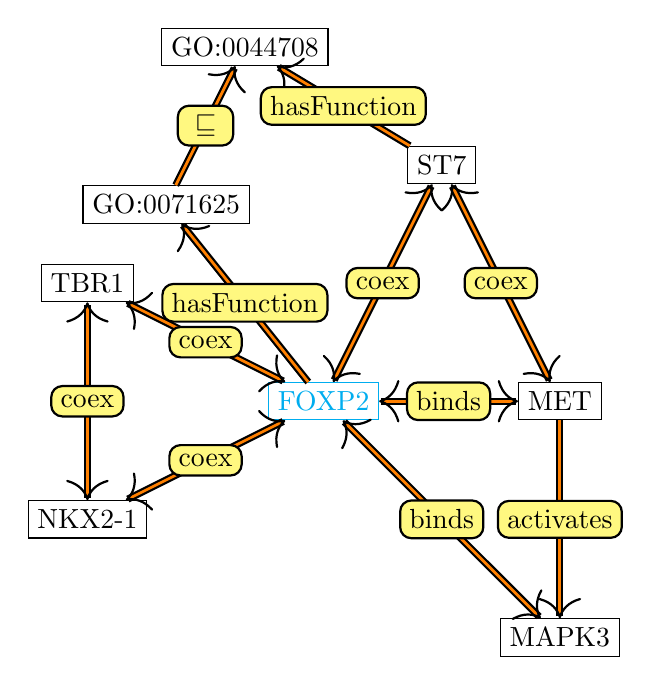
\begin{tikzpicture}
%          \SetUpEdge[lw = 1pt, color = black]
          \GraphInit[vstyle=Shade]
          \tikzset{
            LabelStyle/.style = { rectangle, rounded corners, draw,
              minimum width = 2em, fill = yellow!50,
              text = black },
            VertexStyle/.append style = { inner sep=5pt,
              font = \Large\bfseries},
            EdgeStyle/.append style = {->} }
          
          \SetGraphUnit{5}
          % \tikzset{VertexStyle/.append style={fill}}
          % \tikzset{EdgeStyle/.style={->}}
          \node[draw, color=cyan] (FOXP2) at (0,0) {FOXP2};
          \node[draw] (MET) at (3,0) {MET};
          \node[draw] (ST7) at (1.5,3) {ST7};
          \node[draw] (MAPK3) at (3,-3) {MAPK3};
          \node[draw] (GO0071625) at (-2,2.5) {GO:0071625};
          \node[draw] (GO0044708) at (-1,4.5) {GO:0044708};
          \node[draw] (TBR1) at (-3,1.5) {TBR1};
          \node[draw] (NKX2-1) at (-3,-1.5) {NKX2-1};
          \begin{scope}[/tikz/handle active characters in nodes=false]
          \Edge[label=activates](MET)(MAPK3)
          \Edge[label=hasFunction](FOXP2)(GO0071625)
          \Edge[label=hasFunction](ST7)(GO0044708)
          \Edge[label=$\sqsubseteq$](GO0071625)(GO0044708)

          \tikzset{EdgeStyle/.append style={<->}}
          \Edge[label=binds](FOXP2)(MET)
          \Edge[label=binds](FOXP2)(MAPK3)
          \Edge[label=coex](FOXP2)(TBR1)
          \Edge[label=coex](FOXP2)(NKX2-1)
          \Edge[label=coex](FOXP2)(ST7)
          \Edge[label=coex](MET)(ST7)
          \Edge[label=coex](NKX2-1)(TBR1)
          \end{scope}
          % \tikzset{EdgeStyle/.style={->}}
          % \Edge[label=hf](FOXP2)(GO0044708)
          % \draw[label=binds] (FOXP2) to (MET);
          % \Edge[label=binds](FOXP2)(MET)
          % \Edge[label=activates](MET)(MAPK3)
          % \Edge[label=coexpressed-with](FOXP2)(FOXP4)

          
        \end{tikzpicture}
      }
    \end{column}
    \begin{column}{.4\textwidth}
      \begin{itemize}
      \item FOXP2 + binds - MET = 0
      \item MAP + activates - MAPK3 = 0
      \item MET + binds - FOXP2 = 0
      \item ST7 + hasFunction - {\tt GO:0044708} = 0
      \item ...
      \end{itemize}
    \end{column}
  \end{columns}
\end{frame}

% \begin{frame}
%   \frametitle{Translating embeddings}
%   \centerline{\includegraphics[width=1\textwidth]{transe-algorithm.png}}

%   {\tiny Bordes et al. (2013). Translating Embeddings for
%     Modeling Multi-relational Data.}
% \end{frame}

\begin{frame}
  \frametitle{Some properties of TransE}
  \begin{itemize}
   
  \item graph-based
    \begin{itemize}
    \item works well on RDF graphs
    \item and ontology graphs
    \end{itemize}

    \pause
  \item 1:1 relations only
    \begin{itemize}
    \item not suitable for hierarchies (1-N relations)
    \item not suitable for N-N relations
    \item no transitive, symmetric, reflexive relations
    \end{itemize}
  \end{itemize}
\end{frame}

\begin{frame}
  
  \frametitle{Translating embeddings}

  TransH deals with the 1-N, N-1 and N-N relationships

  \begin{columns}[c]
    \column{.5\textwidth}
      \begin{figure}[h]
        \centering
        \includegraphics[width = 0.6\textwidth]{transe-figure.png}
        \caption{TransE representation}
      \end{figure}


    \column{.5\textwidth}
      \begin{figure}[h]
        \centering
        \includegraphics[width = 0.8\textwidth]{transh-figure.png}
        \caption{TransH representation}
      \end{figure}
      
    
  \end{columns}

%  \centerline{\includegraphics[width=.6\textwidth]{transh-figure.png}}
\end{frame}

\begin{frame}
  \frametitle{Translating embeddings}

  TransR: each relation has its own semantic space.
  
  \centerline{\includegraphics[width=.6\textwidth]{transr-figure.png}}
\end{frame}


% \begin{frame}
%   \frametitle{Translating embeddings}
%   \centerline{\includegraphics[width=\textwidth]{loss-functions-kg.png}}
%   {\tiny Wang et al. Knowledge Graph Embedding: A Survey ofApproaches and Applications.}
% \end{frame}

\begin{frame}
  \frametitle{PyKEEN}
  \begin{itemize}
  \item Python package to generate knowledge graph embeddings
  \item supports many different graph embedding types: TransE, TransH, TransR,
    TransD, RESCAL, etc.
%  \item hyperparameter optimization (``HPO'') and evaluation included
%  \item \url{https://github.com/SmartDataAnalytics/PyKEEN}

  \item mOWL integration
  \end{itemize}
\end{frame}




% \begin{frame}
%   \frametitle{Some limitations}
%   \begin{itemize}
%   \item graph-based (same as random walks):
%     \begin{itemize}
%     \item ontologies are not graphs!
%     \item converting ontologies to graphs loses information
%     \item no axioms, no definitions
%     \end{itemize}
%   \item (this also holds for Graph Convolutional Networks, which are
%     not covered here)
%   \end{itemize}
% \end{frame}


%------------------------------------------------

\begin{frame}
\Huge{\centerline{The End}}
\end{frame}

%----------------------------------------------------------------------------------------

\end{document} 